\chapter{Evaluation}\label{chapter:evaluation}

In this chapter we will evaluate the architectures described in chapter \ref{chapter:architectures} with the method described in chapter \ref{chapter:design_of_experiments}. MEC and Cloudlets will additionally be evaluated with the implementation from chapter \ref{chapter:implementation}. Finally, an introduction to The Near-Far Computing Model will be given.






\section{Assumptions and Clarifications}
\subsection{Bandwidth}
When evaluating, we are making some assumptions about bandwidth. Table \ref{tab:Bandwidth_latency} shows latency and bandwidth for different technologies. The WiFi bandwidths are based on data from CenturyLink\cite{noauthor_24_nodate}. The 4G and 5G bandwidths are real-world examples from 4g.co.uk\cite{noauthor_how_nodate}. The 4G latency is from ping tests, while the 5G latency is from Verizon\cite{noauthor_what_2020}.
\renewcommand{\arraystretch}{1.2}
\begin{table}[h!]
    \centering
    \begin{tabular}[c]{l|p{3cm}p{4cm}}

        Technology & Latency (ms) & Bandwidth (Mbps) Download/Upload \\
        \hline

        Wifi (2.4GHz) & <=1 & 150/150  \\

        Wifi (5GHz) & <=1 & 450/450  \\

        4G & 30-65 & 42/25  \\

        5G & 30 & 200/100  \\

        Wired LAN & <=1 & 1000+/1000+  \\

        WAN & 10-300+ & 1000+/1000+  \\

        
        
    \end{tabular}
    \caption{Latency and bandwidth for different technologies.}
    \label{tab:Bandwidth_latency}
\end{table}
When doing calculations about overhead in this chapter, we will be using numbers from table \ref{tab:Bandwidth_latency}.





\subsection{Hardware}
According to cpubenchmark\cite{noauthor_passmark_nodate}, flagship phones are about half as fast as a standard desktop CPU. We assume that we are dealing with below-average cellphone CPUs, as most people do not have the flagship phone. We will test the different strengths of the MEC Server. We assume that the data center will have plenty of resources. 


\subsection{Parameters}
On the tables shown in this chapter, the type of parameters will be on the left row while the actual parameters will be on the right.
\renewcommand{\arraystretch}{1.5}
\begin{table}[h!]
    \centering
    \begin{tabular}{l|p{12cm}}
        
        Parameter &  Meaning\\
        \hline
        Node type & Describes the type of node we are showing for this column. \\

        Limitation & A limit on how many iterations the node can do per second. \\

        Iterations & The number of iterations done by the node. \\

        RTT to Local (ms) & Latency between the Local node and the Near or Far node. \\
        
        Frequency & How often we communicate with the Local node. If it is 10, then we get information from the Local node every 10th iteration. \\
        \hline
        \textbf{Time used (s)} & The time used for calculating the number of iterations given. This is in other words the final results. \\
    \end{tabular}
    \caption{Explanation of parameters and results.}
    \label{tab:parameter_explanation}
\end{table}
\renewcommand{\arraystretch}{1.2}

Table \ref{tab:parameter_explanation} describes what each of the parameters and result means. Note that results are written in bold text.

%Move to implementation?

\subsection{Local Execution}
%lacking geographic location?
\begin{table}[h!]
    \centering
    \begin{tabular}[c]{c|p{2cm}}

        Node type & Local \\

        Limitation          & 30  \\

        Iterations          & 10000  \\

        RTT to Local (ms)   & 0  \\

        Frequency           & 1 \\

        \hline
        \textbf{Time used (s)} & \textbf{333.6} \\

    \end{tabular}
    \caption{Only Local execution.}
    \label{tab:local_execution}
\end{table}
Table \ref{tab:local_execution} shows the time used for local execution only. We show this to be able to compare with offloading results, and to see if there is significant speedup.

\subsection{Redundant Measurements}
We argue that due to the high-level nature of our prototype, we will have close to the same parameters for Google Anthos, Amazon Cloudfront, and Akamai as with either MEC or Cloudlets. Therefore we do not present prototype results for these architectures, as they are redundant.

\subsection{Iterations}
To best show how each node performs, we have divided a workload over each type of node. This workload will consist of 10000 iterations.





\section{Multi-Access Edge Computing} \label{section:MEC_evaluation}
This section will show results of testing with the prototype for MEC, and then discuss these results. Additionally it will point out characteristics for this architecture.

\subsection{Full offloading}




\begin{table}[h!]
    \centering
    \begin{tabular}[c]{|c||p{2cm}|p{2cm}|p{2cm}|}
        \hline
        Node type & Local & Near & Far \\
        \hline
        Limitation          & 30 & 100 & 300  \\
        \hline
        Iterations          & 0 & 900 & 9100  \\
        \hline
        RTT to Local (ms)   & 0 & 30 & 170 \\
        \hline
        Frequency           & 1 & 1 & 80 \\
        \hline
        \hline
        \hline
        \textbf{Time used (s)}       & \textbf{0} & \textbf{29.2} & \textbf{30.2} \\
        \hline
    \end{tabular}
    \caption{Full offloading}
    \label{tab:MEC_full_offloading_low_frequency}
\end{table}

Table \ref{tab:MEC_full_offloading_low_frequency} shows the result of full offloading with low frequency of communication with the Far-Node.






\subsection{Partial offloading}



\begin{table}[h!]
    \centering
    \begin{tabular}[c]{|c||p{2cm}|p{2cm}|p{2cm}|}
        \hline
        Node type & Local & Near & Far \\
        \hline
        Limitation          & 30 & 100 & 300  \\
        \hline
        Iterations          & 850 & 850 & 8300  \\
        \hline
        RTT to Local (ms)   & 0 & 30 & 170 \\
        \hline
        Frequency           & 1 & 1 & 80 \\
        \hline
        \hline
        \hline
        \textbf{Time used (s)}       & \textbf{28.0} & \textbf{29.8} & \textbf{28.0} \\
        \hline
    \end{tabular}
    \caption{Partial offloading}
    \label{tab:MEC_partial_offloading_low_frequency}
\end{table}

Table \ref{tab:MEC_partial_offloading_low_frequency} shows the result of partial offloading where the Far node is doing most of the work. Frequency of communication between Local or Near node and Far node is low. 


\begin{figure}[t]
    \centering
    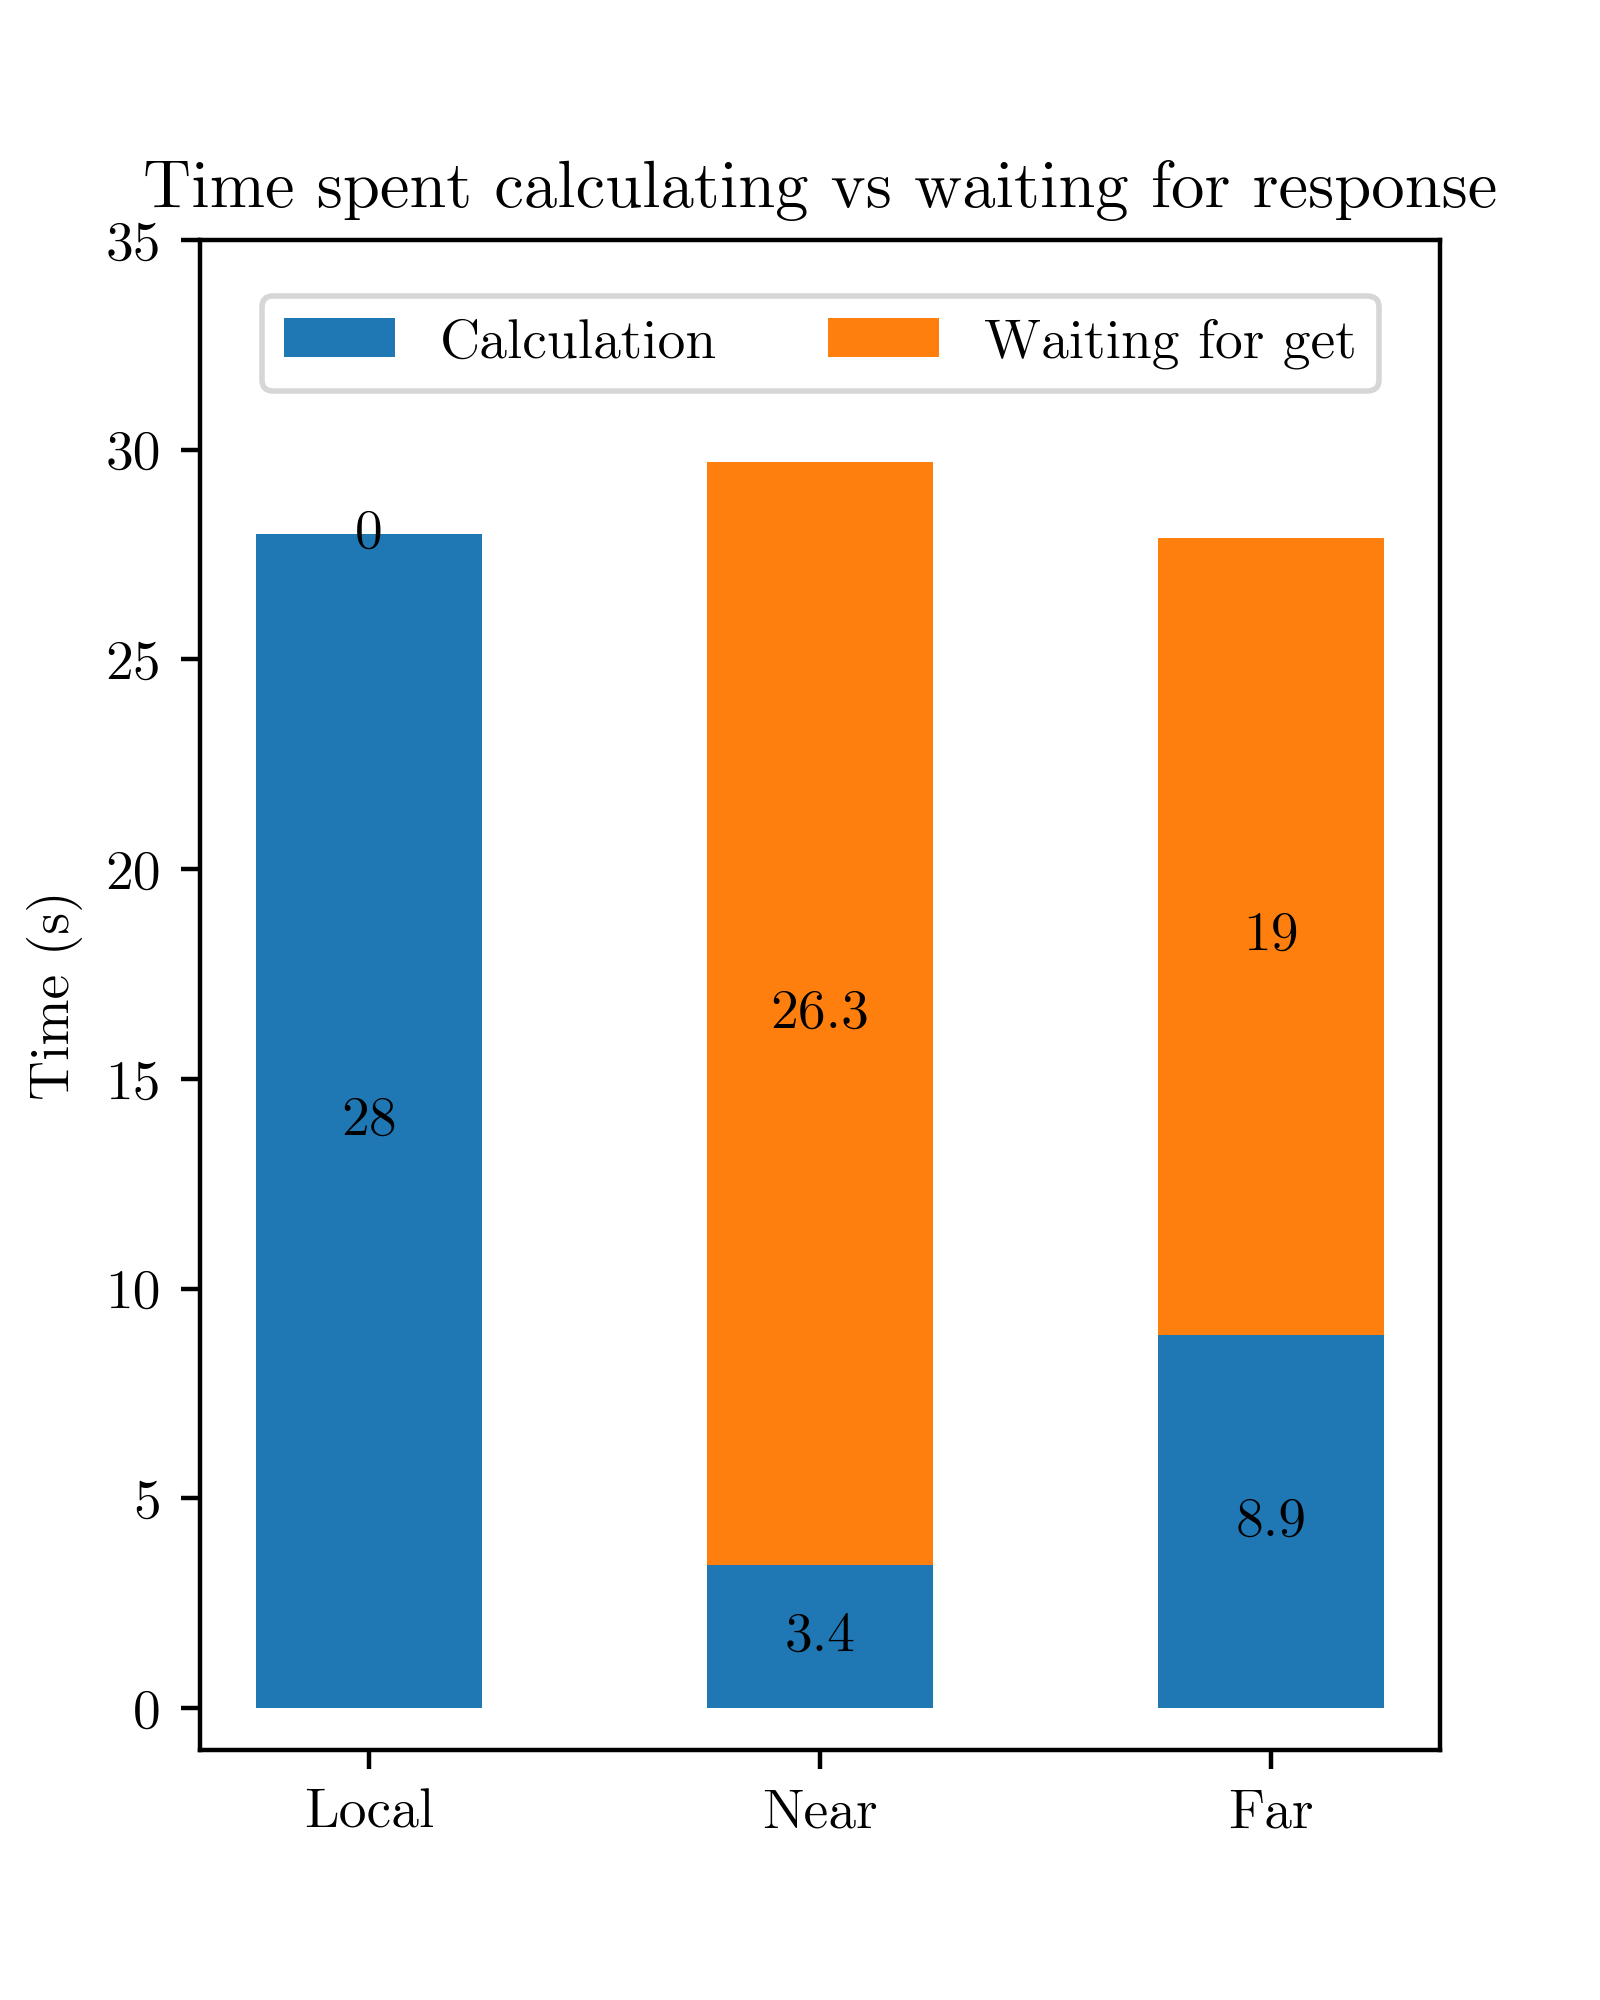
\includegraphics[scale=1]{chapters/6_evaluation/figures/MEC_Partial_bar.png}
    \caption{Illustration of how much time is spent on waiting for data due to latency when using MEC Server.}
    \label{fig:MEC_partial_bar}
\end{figure}

Figure \ref{fig:MEC_partial_bar} shows how latency affect the the total time used when we have to constantly get data from the local device. It uses the same configuration as shown in table \ref{tab:MEC_partial_offloading_low_frequency}.





\subsection{Characteristics}

\subsubsection{Control}
As discussed in section \ref{section:MEC_architecture}, the network architecture of MEC is up to the programmers. They can use NFV and SDN to control how each mobile device will be able to use the architecture. They can in other words use SDN and NFV to tailor the network to the context. Since VMs can be uploaded to surrounding MEC Servers, ensuring good \textit{relocation transparency} should be trivial. Due to SDN and NFV they could quickly redirect packets to new MEC Server when needed. The level of \textit{migration transparency} is therefore also left to developers.

\subsubsection{Offloading}
Since they use the cellular network to offload work, this architecture is well suited for IoT devices that can afford the latency. The cellular network is ubiquitous in modern society, and therefore it is optimal for IoT devices that move a lot, e.g. self-driving cars. When offloading they have to upload something, e.g. a VM, to the MEC Server. Alternatively they can make the MEC Server download from elsewhere. Since MEC uses VMs on the servers when offloading, the level of \textit{access transparency} is very good. The VMs ensure that the APIs for all the nodes are the same. Since cellular networks cover such a large area, \textit{location transparency} is trivial as the device can move quite a lot of distance before any migration is needed. If a node were to fail, it is up to the developers to ensure that other resources are available to recover from the failure. In other words, the level of \textit{failure transparency} is up to the programmers.

\subsubsection{Deployment}
MEC is easily horizontally scalable, as more MEC Servers can easily be added to cell towers. The only limit is how much power there is available and how much space there is available. If only a few servers is needed, then the cost is not too high either. It is also easily scalable in the sense that you can add more VMs to the MEC Server to help with offloading if needed. Another benefit of using VMs is that \textit{concurrency transparency} is easy to ensure as long as the MEC Server does not run out of resources. This is because they are in sperate VMs and should not affect each other.



%offloading
%    compute 
%    storage
%distribution
%    scaling
%Control


%tabell? subsections? idk

%TODO
% Gjøre målinger med overføring av filer først. Finn data på bandwidth og pluss det på tiden.
% Gjøre målinger hvor det kreves mer samhandling mellom nodene. Vi må se latency!


%\cite{mach_mobile_2017} for hvor mye som skal offloades.!!!!
% test med 100% offload, 50% offload osv
%\begin{itemize}
 %   \item Easily scalable as we have the common interface. This makes it easy to add more vms to run more apps. So, its horizontally scalable?
%\end{itemize}





% -------------------------------------------------------------------------------------------





\section{Cloudlets}

This section will show results of testing with the prototype for Cloudlets, and then discuss these results. Additionally it will point out characteristics for this architecture.


\subsection{Full execution}


\begin{table}[h!]
    \centering
    \begin{tabular}[c]{c|p{2cm}p{2cm}p{2cm}}

        Node type & Local & Near & Far \\

        Limitation          & 30 & 100 & 300  \\

        Iterations          & 0 & 2500 & 7500  \\

        RTT to Local (ms)   & 0 & 3 & 170 \\

        Frequency           & 1 & 1 & 80 \\

        \hline
        \textbf{Time used (s)}       & \textbf{0} & \textbf{26.2} & \textbf{25.4} \\

    \end{tabular}
    \caption{Full offloading with low frequency of communication between Local and Near/Far.}
    \label{tab:Cloudlet_full_offloading_low_frequency}
\end{table}

Table \ref{tab:Cloudlet_full_offloading_low_frequency} shows the result of Full offloading to a nearby Cloudlet with low frequency of communication with Far node.







\subsection{Partial offloading}



\begin{table}[h!]
    \centering
    \begin{tabular}[c]{c|p{2cm}p{2cm}p{2cm}}

        Node type & Local & Near & Far \\

        Limitation          & 30 & 100 & 300  \\

        Iterations          & 700 & 2500 & 6800 \\

        RTT to Local (ms)   & 0 & 3 & 170 \\

        Frequency           & 1 & 1 & 80 \\

        \hline
        \textbf{Time used (s)}       & \textbf{23.0} & \textbf{24.3} & \textbf{22.5} \\

    \end{tabular}
    \caption{Partial offloading with low frequency of communication between Local and Near/Far.}
    \label{tab:Cloudlet_partial_offloading_low_frequency}
\end{table}




\begin{figure}[t]
    \centering
    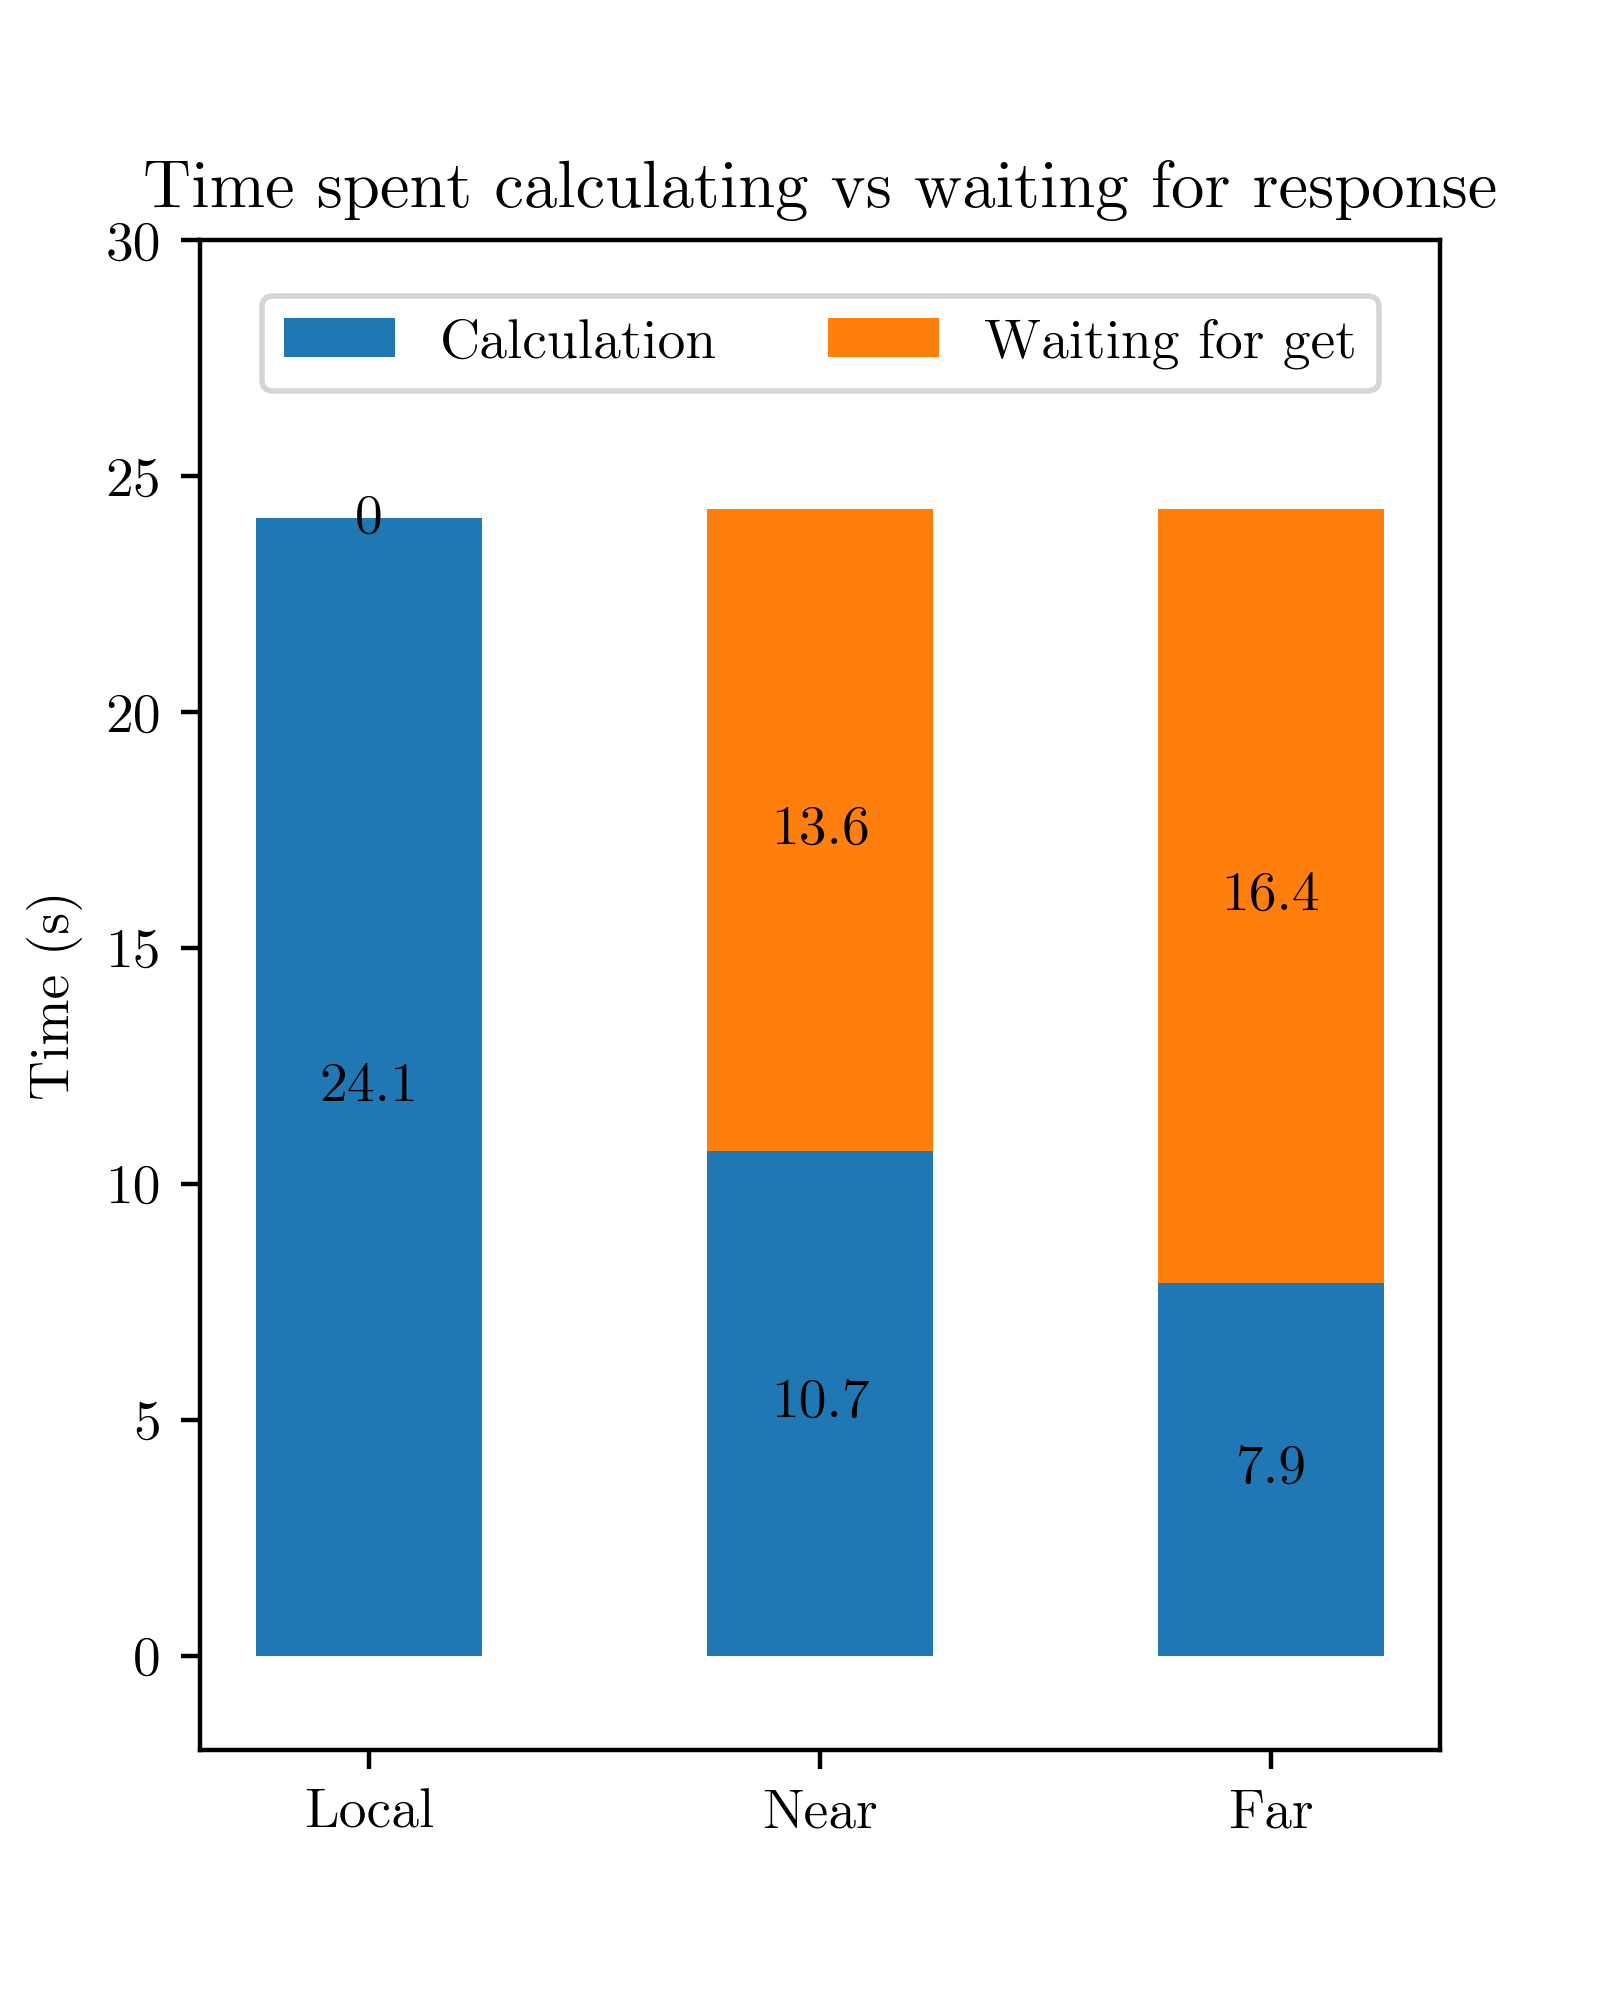
\includegraphics[scale=1]{chapters/6_evaluation/figures/bar_local_near_far_compare_low_interaction.png}
    \caption{Illustration of how much time is spent on waiting for data due to latency when using Cloudlets.}
    \label{fig:Cloudlet_latency_bar}
\end{figure}
Figure \ref{fig:Cloudlet_latency_bar} shows how much time used on waiting for data from Local, compared to how much time is used on calculating. The configuration used here is the same as shown in table \ref{tab:Cloudlet_partial_offloading_low_frequency}.




\subsection{Characteristics}
\subsubsection{Control}
Controlling Cloudlets is done by the owner of each Cloudlet. Since Cloudlets are to be placed on locations, e.g. a coffee shop, then the owner of that location is able to configure the Cloudlet. The location owner can then limit usage and limit what kinds of applications are used on the Cloudlet. Handling failure and having good \textit{failure transparency} is mostly up to the programmer in Cloudlets. Should the Cloudlet fail, then a different near Cloudlet should take over, or in the worst case let the Local device handle it. 

\subsubsection{Offloading}
Cloudlets use \textit{dynamic VM synthesis} \cite{satyanarayanan_case_2009} to offload work. Essentially it means that we have to give the Cloudlet a VM to run the application. This makes \textit{access transparency} for Cloudlets quite good in theory. However, it gives an overhead which they reported to be quite high. This has likely been improved since 2009 as technology has improved. Bandwidth, storage and computational power have significantly improved, which mitigates many of the issues they raised.

\subsubsection{Deployment}
Distribution is expensive for Cloudlets. Satyanarayanan et al\cite{satyanarayanan_case_2009} purposes different payment models, but each owner of a location has to decide if it is worth the investment. Since they are supposed to be ubiquitous, the total cost of having these readily available everywhere in society will be significant. If the Cloudlets are ubuiquitus, then the level of \textit{location and relocation transparency} is quite high. In their paper, they purpose a way of seamlessly migrating to other Cloudlets when needed. If this is accomplished, then the users of the local devices will not notice any drop in performance. Due to the ubiquitous nature of Cloudlets, having \textit{concurrency transparency} should not be a problem. Overloading all of the nearby Cloudlets will be a rare occurrence due to their ubiquitous nature.





% -------------------------------------------------------------------------------------------







\section{Google Anthos}
\subsection{Characteristics}
\subsubsection{Control}
Controlling the Anthos architecture is relatively easy as GCP will take care of all the difficult parts. A client can control all the nodes in the Anthos control panel. This means that the one who owns the GCP account has full control over the nodes. The level of \textit{access transparency} is quite high, as Anthos will take care of all the low-level problems. It is up to the programmer to decide how containers running on the platform will communicate. It is also up to the programmer to decide whether they want users to be able to relocate objects. In other words \textit{migration transparency} decided by the programmers.

\subsubsection{Offloading}
Since Anthos uses containers, offloading can be quite straightforward. It is the programmers who decide how offloading will work. Essentially, the Local device only needs to somehow contact the on-premises machines, for example through WiFi and LAN connections, to offload. The level of \textit{location transparency} is up to the programmers. It is dependent on how the containers are set up. Kubernetes can be set up to manage \textit{replication and concurrency transparency}, as it lets you configure where the containers should reside and how many of them should be there, as well as many other parameters.

\subsubsection{Deployment}
Deploying is relatively simple. As discussed earlier, a client only needs to install Anthos software on on-premises hardware and then configure Kubernetes to use it. Ensuring \textit{failure transparency} can be challenging, but Kubernetes can be configured to handle failures. Essentially, it is up to the programmer to decide what happens if one occurs.





% -------------------------------------------------------------------------------------------







\section{Amazon Cloudfront}
\subsection{Characteristics}
\subsubsection{Control}
Controlling Cloudfront is done in the Cloudfront control panel in the AWS console. Cloudfront allows clients to set up a wide array of features for their architecture. They provide DNS, NFV, Lambda@edge, security, certificates, et cetera. All of this is controlled by the programmers in the AWS console.  


\subsubsection{Offloading}
With AWS, clients can set up servers, container software, or Lambda@edge on Cloudfront. This gives much freedom to the programmers on how they will set up the architecture. A downside of using AWS Lambda is something called warm-up time. It is quite small, but can be noticed in extreme latency-aware contexts. The warm-up time depends on the programming language used, but it comes in addition to the latency towards the edge location. When it comes to \textit{concurrency, location}, and \textit{replication transparency}, it is up to the programmer, but they are very easily adjustable. For example, for AWS Lambda, a single parameter can be changed to let it scale more. AWS will handle scaling, and the programmer will only need to set the limit. When using servers clients have to add more servers to scale out. It is not automatically done. The level of \textit{access transparency} is high due to containerization and AWS Lambda. However, if servers are used, then the programmer has control of the access transparency level. \textit{Relocation and migration transparency} can be ensured by Cloudfront, unless you use the servers. Then it is up to the programmer to control it. 


\subsubsection{Deployment}
When setting up Cloudfront, clients do it through the AWS control panel. They are limited to use the edge servers that AWS provides. These servers are deployed all over the world. Nonetheless, in some places, there might be a long distance to the nearest server. Ensuring \textit{failure transparency} is handled by Cloudfront in this architecture. The programmer can focus more on what the program should do rather than what happens if it fails. 




% -------------------------------------------------------------------------------------------





\section{Akamai}
\subsection{Characteristics}
\subsubsection{Control}
Akamai features are controlled through Akamai's console. The level of \textit{access and migration transparency} is decided by the programmer in this architecture.

\subsubsection{Offloading}
Akamai does offer ways of offloading, but they focus more on bringing content to the edge rather than computation alone. Caching is the primary purpose of Akamai edge servers, and using their edge servers for this, ensures \textit{location, relocation, replication, and concurrency transparency}. The level of \textit{replication transparency} is also somewhat up to the programmer, as they can choose the locations of where to cache the content.

\subsubsection{Deployment}
Setting up the edge servers is done through Akamai's console. Clients set up the edge server where they want it and then push their content to that server. Akamai will take care of eventual failures and route requests to the original server if needed. This ensures \textit{failure transparency}. However, if the original server is very distant, the client will most likely notice a drop in performance or response time.


% -------------------------------------------------------------------------------------------




\section{Discussion of Findings}
In this section, we will discuss the results from the previous sections. 
%introduction

% Adding extra Near Nodes or Far nodes will in our prototype and dividing the work between them will give T/n better time. 

\subsection{Comparing Cloudlets and MEC}
The results show us that if enough funding is available, then Cloudlets gives the best result. Having low latency between Local and Near, like the Cloudlet, is preferable in order to obtain better results. Yet, one could argue that installing MEC Servers is significantly less complicated and cheaper as clients only have to install them at base stations that cover a wide area. It is significantly easier for MEC when it comes to migration due to how much area is covered with cellular. If the mobile device were to move in the Cloudlet architecture, then Cloudlets should already be ready to offload in the new location. This is hard because it can be difficult to decide which Cloudlet to migrate to, before it is too late. Since MEC covers such a large area, it should not be a problem to see when it is needed to migrate to other base stations. However, migration in MEC will likely take a longer time, as Cloudlets often will be on the same LAN and can therefore transfer faster and more reliably.




\subsubsection{Results}

\begin{table}[]
    \centering
    \begin{tabular}{c|c}

       Type  & Total time used (s)\\
       \hline

       Local execution                         & 333.6  \\

       MEC Full offloading       & 30.2 \\

       MEC Partial offloading    & 29.8 \\

       Cloudlets Full offloading & 26.2 \\
 
       Cloudlets Partial offloading  & 24.3 \\

    \end{tabular}
    \caption{Summary of time used when offloading, compared to Local execution only}
    \label{tab:total_time_compare}
\end{table}
Table \ref{tab:total_time_compare} shows the time used for all the tests. To clarify, since Local, Near and Far work in parallel, the time used in the table is represented by the node who used the longest time. We observe that there is not much difference in results when comparing Full offloading and Partial offloading. Nonetheless, Partial offloading unsurprisingly has the best results.

Full offloading might, for some devices, be a requirement. The two most likely reasons for this is if the Local device has minimal computational power or needs to save battery. Therefore, one should not always choose Partial offloading. When deciding on what to use, one should consider the context. For instance, if battery life is the most crucial factor, then using Full offloading is preferred. Our tests only show the result of focusing on performance and the least used time. However, one can change most of the parameters to address other needs of the context. For example, if the work is very latency-sensitive, the parameters can be modified to offload more to the Near nodes than the Far nodes if more Near nodes are available.



\subsubsection{Decreasing interaction}
Figure \ref{fig:MEC_partial_bar} and \ref{fig:Cloudlet_latency_bar} illustrates how much time is used on waiting for a response from the Local node. Since the Far node communicates less, we can see that it gets more computational time than the Near node. 


\begin{figure}
    \centering
    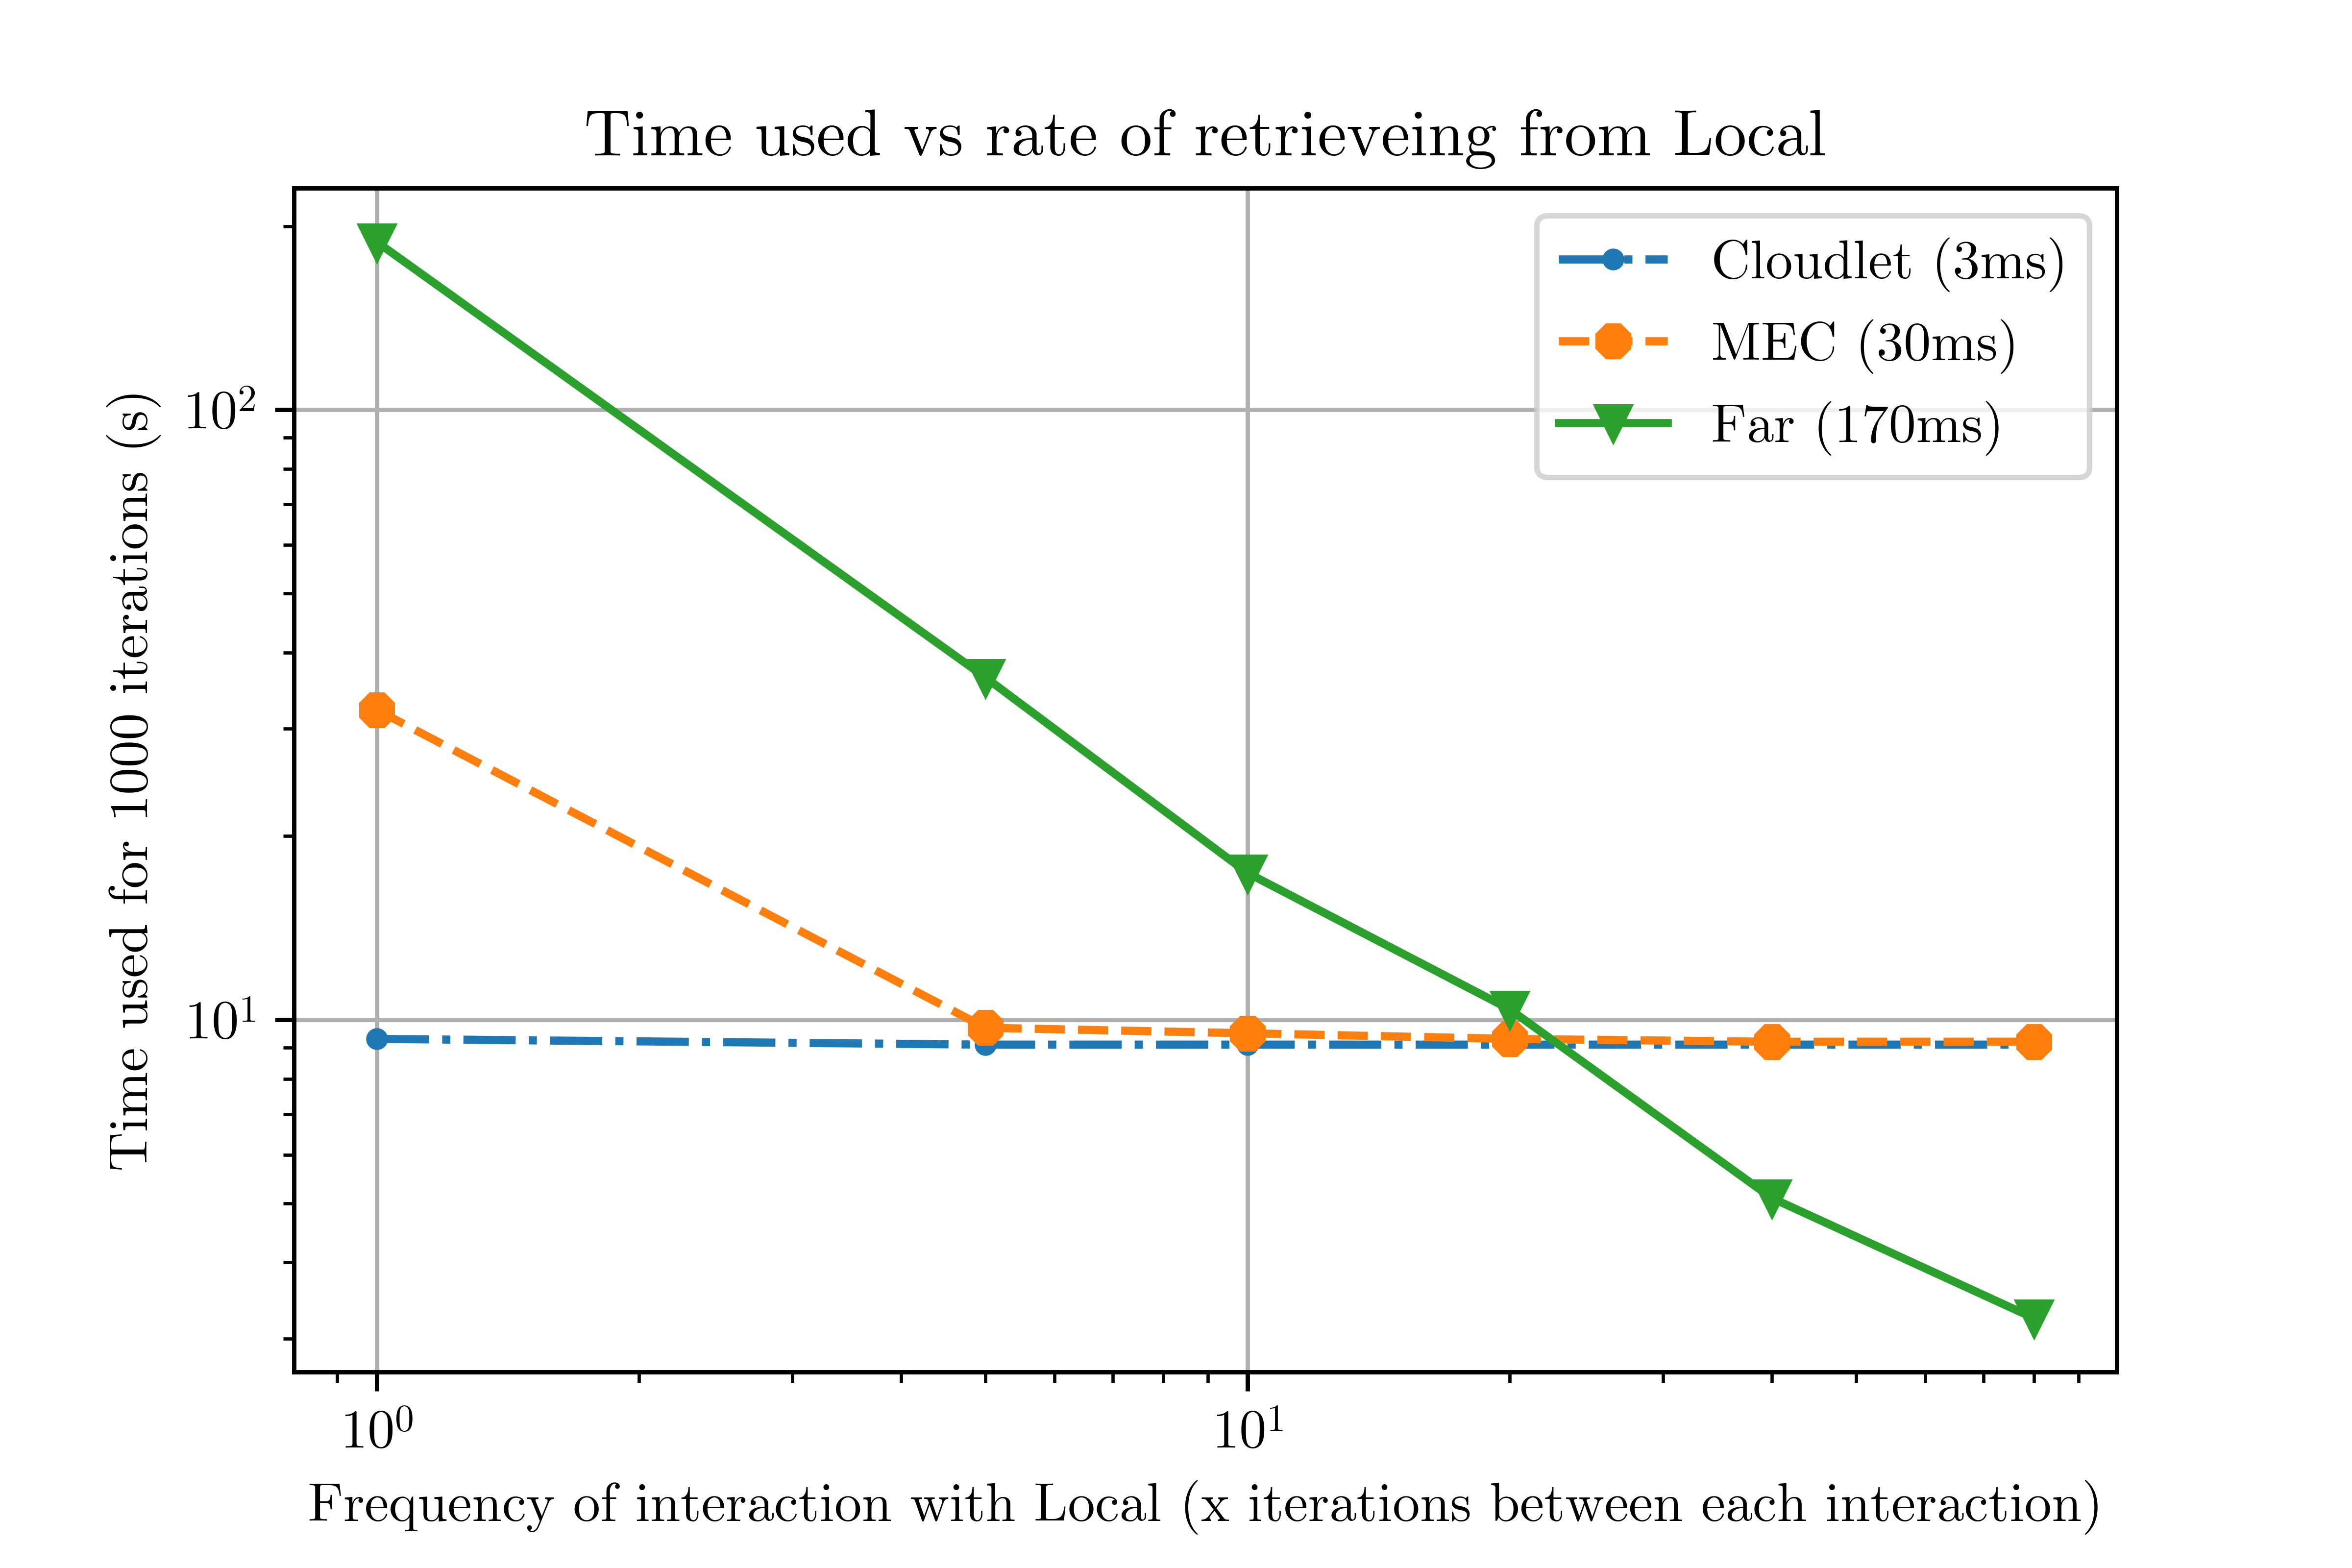
\includegraphics{chapters/6_evaluation/figures/All_latency.png}
    \caption{Illustration of how decreasing interaction improves performance.}
    \label{fig:all_graph_decrease}
\end{figure}

Figure \ref{fig:all_graph_decrease} illustrates how decreasing communication with Local will yield better results for each type of node. However, both MEC and Cloudlet stagnate as limited processing power becomes the bottleneck. This means that when frequent communication is needed, one should use the Near node. The Far node is best to take care of work that does not require frequent communication. As we can see in figure \ref{fig:all_graph_decrease}, we get much faster results with the Far node when the frequency of interaction is high, compared to the Near nodes.





\subsubsection{Horizontal scaling}
The results shown for MEC and Cloudlets have just one HashWorker per node. This is to show the viability of Near-Far Computing in a simple isolated form. Nonetheless, one can easily horizontally scale the amount of workers and nodes. If the workload is as parallelizable as our hashing setup, then adding nodes or workers will give significantly better times, assuming that they get the same resources.


\subsubsection{Overhead}
In the Emerald environment, there is very little overhead compared to overheads in a real-life context. When running Emerald, only a few objects need to be replicated or transferred instead of a whole VM or container. In other, more real-life environments, we argue that the response time can be affected by such replications or transferals, but that this can be mitigated by understanding the context and pre-loading the environment onto the Near nodes. This overhead usually consists of transfer time plus starting time. The transfer time is mainly affected by bandwidth. By looking at table \ref{tab:Bandwidth_latency} we can see that it is preferable to use WiFi rather than cellular, as WiFi has higher bandwidth.








\section{The Near-Far Computing Model}
In this section, we will discuss the characteristics of The Near-Far Computing Model and give an introduction to it. 


%The Near-Far Computing Model is best utilized when you can have a Near node doing latency critical work, and a Far node doing other work that does not require a real-time response. For example, if the Local device is a smart device that need quick response on their data, it can offload to the Near node. When the Near node is done calculating, it can use the Far server to analyze the result as well as logging it, while the Local device can use the calculated data for responding to the context. For storage, Near-Far is great for caching. Having caches that is closer to the client will result in way quicker results.

%The common thing for all the discussed architectures is that they use a mix of both edge nodes and server nodes. They try as best as possible to use the edge nodes, but the distant strong data centers can aid when needed. 

%If the Near node were to fail, then the Far node can take over. However, due to latency the Far node will give the client a worse experience if response time is critical. This is process is the same as discussed in article The Case for VM-Based Cloudlets in Mobile Computing\cite{satyanarayanan_case_2009}.

\subsection{Distribution Transparency}
In the following subsections, we will discuss distribution transparency in Near-Far Computing.

\subsubsection{Access Transparency}
When using The Near-Far Computing Model, one should use containerization or VMs to provide common API or middleware for all the nodes in the system. This ensures that developers do not have to deal with very low-level programming and focus more on providing features and solutions. This solution is one thing that most of the discussed architectures have in common.

\subsubsection{Location Transparency}
Location transparency determined by the programmer, but one should try to hide where objects are located in most cases. Usage of Near nodes will allow programmers to ensure location transparency due to low latency and how relatively resource-rich they are.

\subsubsection{Relocation Transparency}
Relocation transparency can be difficult if the area where the device is connected to the Near node is not wide. For example, if the device has to connect to a new node each time its owner enters a new room, ensuring relocation transparency can be challenging. However, with good algorithms and enough knowledge about the context, it is possible to ensure perfect relocation transparency. If the connection covers a wide area, like cellular, then relocation is easier since it is less frequent.

\subsubsection{Migration Transparency}
Most of the discussed architectures do not focus on migration transparency. Nonetheless, control is left to the programmers. This means that if the application needs users to control where objects are located in the system, it can be implemented. Yet, we believe that this is needed in very few cases, and hiding where objects are located is much more important to ensure a good experience.

\subsubsection{Replication Transparency}
Replication transparency is up to the programmer. With enough nodes available, the programmer can add or remove objects as they see fit. Most of the architectures are typically hiding where objects are located, so one should ensure that in most cases replication is not noticed.

\subsubsection{Concurrency Transparency}
Concurrency transparency configured by the programmer. In most cases, however, it is best to avoid showing that multiple users are using the same resources. For example, users should not notice that several others are retrieving the same content or querying the same database. 

\subsubsection{Failure Transparency}
If enough nodes are available, then recovering from a failure should have minimal impact on the user. If the application in question is latency-aware and is forced to use Far or Local resources to do these time critical operations, then the client will suffer. However, one should quickly recover to the optimal state, for example, by using checkpoints, like available in Emerald.








\subsection{Introduction to The Near-Far Computing Model}
With the information provided and discussed in the above sections, we can now give an introduction to The Near-Far Computing Model.

The Near-Far Computing Model is a spectrum that covers all models or architectures that focus on mitigating latency issues by using Near nodes and Far nodes. \textit{Near nodes} are edge or fog nodes that provide resource-rich nodes as close as possible to the user to ensure minimal latency. \textit{Far nodes} are distant, extremely scalable, and generally resource-rich nodes that usually reside in data centers that can provide heavy computational power and nearly limitless storage at the cost of latency.

\begin{figure}[t]
    \centering
    %\textbf{The Near-Far spectrum}\par\medskip
    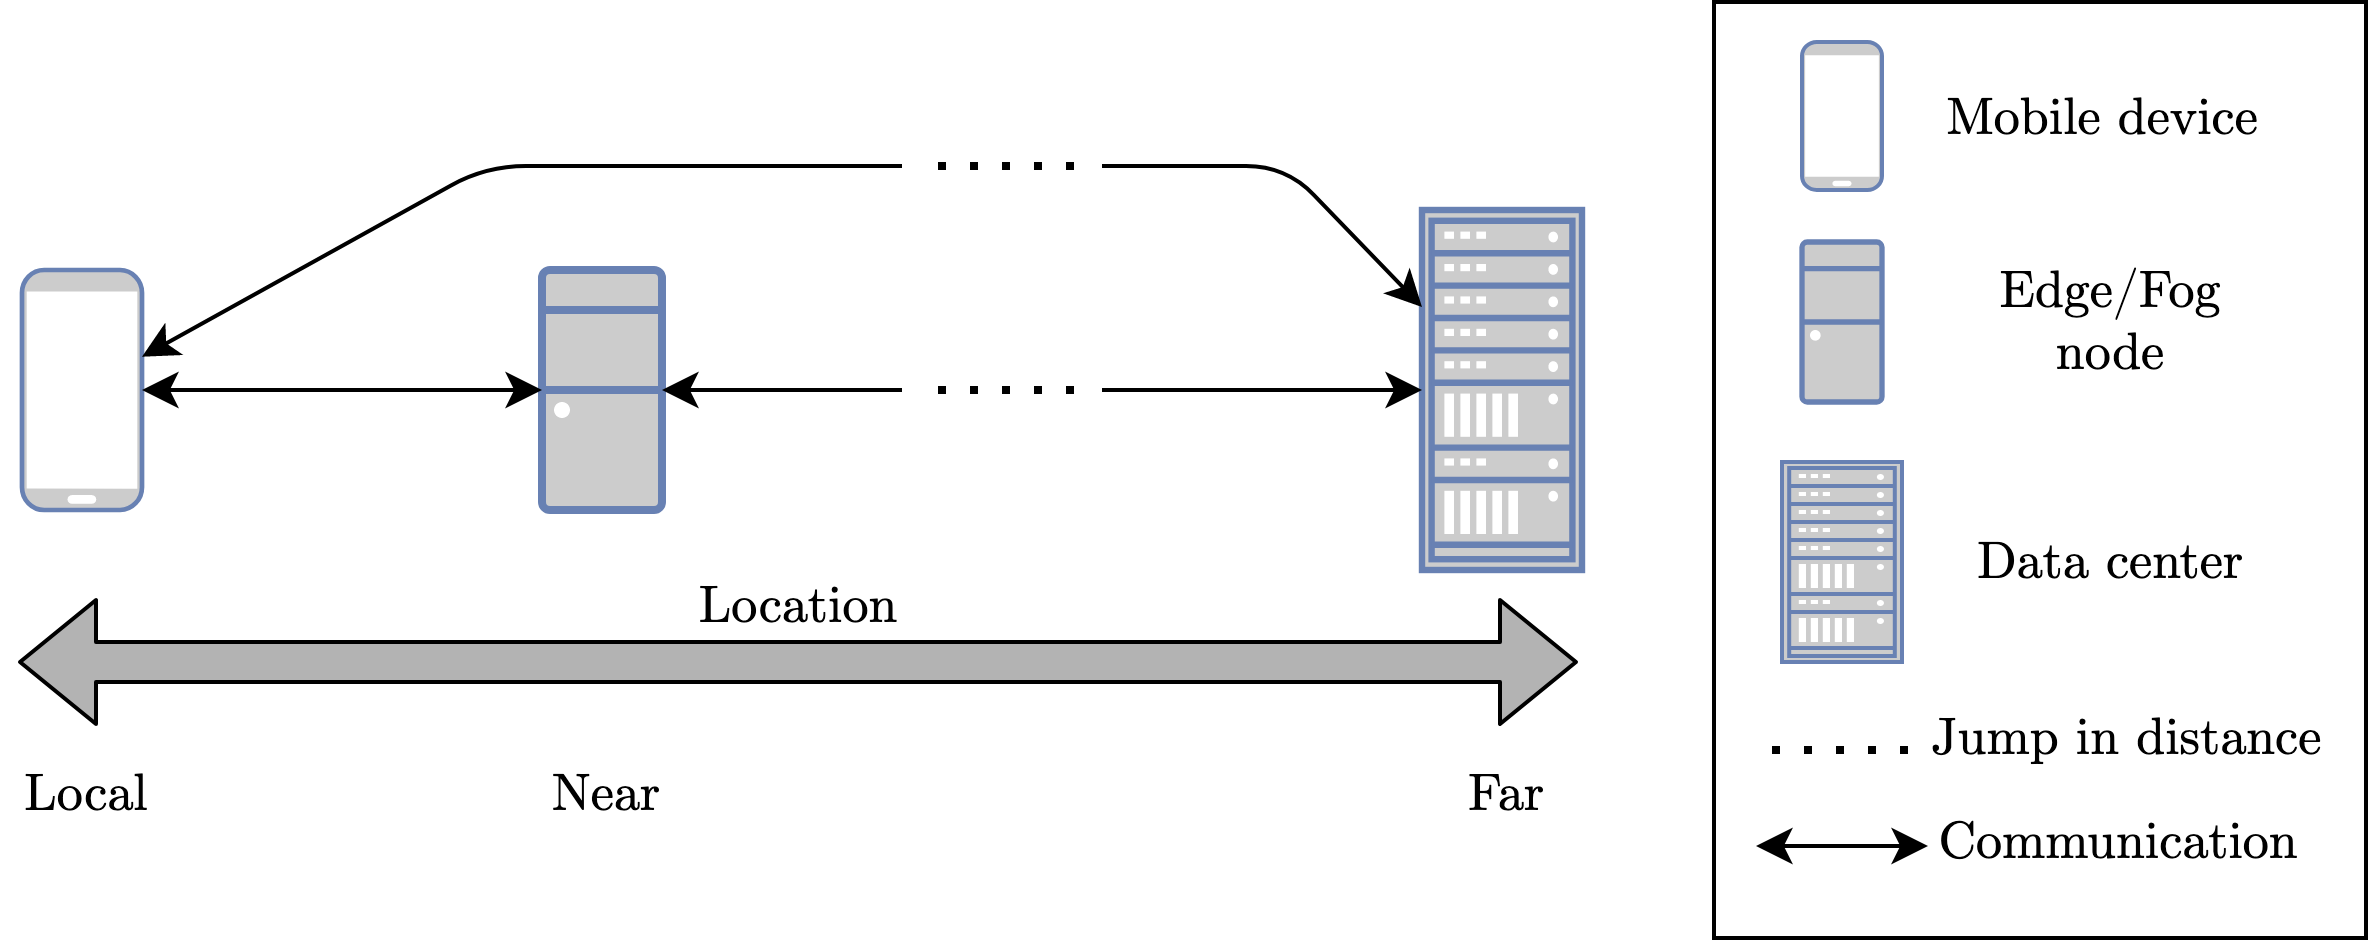
\includegraphics[scale=1]{chapters/6_evaluation/figures/near-far_diagram.png}
    \caption{The Near-Far spectrum}
    \label{fig:nearFarSimple}
\end{figure}


Figure \ref{fig:nearFarSimple} illustrates the Near-Far spectrum. We have a Local device that communicates with a Near device, typically an edge or fog device, e.g., a Cloudlet. This Near node or Local device will communicate with the Far node to offload less time-sensitive work or storage. The Near node should optimally be in close proximity to the Local device to ensure low latency.

\subsubsection{Control}
Since VMs or containers are preferred for offloading, the programmers have much control. This method restricts access to low-level control, but it would, in most cases, not be needed, as enough control is given within the VMs or containers. NFV and SDN can be used to control the network structure when needed.

\subsubsection{Offloading}
One can use the Near node to offload time-sensitive work and further aid this offloading with the strong Far nodes. Therefore, using The Near-Far Computing Model is most applicable when having work or storage that needs to be offloaded with low latency, while at the same time have less time-sensitive parts that can be done on a stronger node that is geographically distant. 

After each use, the nodes should return to their original state by cleaning up the VM or container.


\subsubsection{Deployment}
The closer the Near node is to the Local device, the more expensive it will become to deploy. When deciding on what the requirement is for response time, one has to consider that it can become quite costly to deploy. For example, MEC using nodes at the base of cell towers/base stations will be more scalable and cheaper to deploy than Cloudlets who need to be ubiquitous and deployed almost everywhere. The trade-off is then latency and scalability versus cost. 


\section{Summary}
In this chapter, we have tested MEC and Cloudlets with the program described in implementation. We have also discussed the characteristics of all the architectures. Then, we discussed how these characteristics relate to The Near-Far Computing Model. Finally, we have provided an introduction to The Near-Far Computing Model.





